         \chapter{The particles that substances are made of}\fancyfoot[LO,RE]{Chemistry: Matter and materials}
\label{chap:composition}
    \setcounter{figure}{1}
    \setcounter{subfigure}{1}
    \label{m38120}
\section{Atoms and compounds}
    \subsection*{The atom as the building block of matter}
            \nopagebreak
            \label{m38120*cid2} $ \hspace{-5pt}\begin{array}{cccccccccccc}   \end{array} $ \hspace{2 pt}\raisebox{-5 pt}{
\includegraphics[width=0.5cm]{col11305.imgs/summary_www.png}} {(section shortcode: P10053 )} \par 
      \label{m38120*id307092}We have now seen that different materials have 
different properties. Some materials are metals and some are non-metals; some 
are electrical or thermal conductors, while others are not. Depending on the 
properties of these materials, they can be used in lots of useful applications. 
But what is it exactly that makes up these materials? In other words, if we were 
to break down a material into the parts that make it up, what would we find? And 
how is it that a material's microscopic structure (the small parts that make up 
the material) is able to give it all these different properties?\par 
\begin{minipage}{.6\textwidth}
      \label{m38120*id307099}The answer lies in the smallest building block of 
matter: the \textbf{atom}. It is the \textsl{type} of atoms, and the way in which they are 
\textsl{arranged} in a material, that affects the 
properties of that substance. This is similar to building materials. We can use bricks, steel, cement, wood, straw (thatch), mud and many other things to build structures from. In the same way that the choice of building material affects the properties of the structure, so the atoms that make up matter affect the properties of matter.\par 
\end{minipage}
\begin{minipage}{.4\textwidth}
 \begin{center}
\includegraphics[width=0.6\textwidth]{photos/atom_model_kit.jpg}
 \end{center}
\end{minipage}

      \label{m38120*id307459}It is not often that substances are found in atomic 
form (just as you seldom find a building or structure made from one building material). Normally, atoms are bonded (joined) to other atoms to form \textbf{compounds} or \textbf{molecules}. It is only in the \textsl{noble gases} (e.g. helium, neon and argon) that atoms 
are found individually and are not bonded to other atoms. We looked at some of the 
reasons for this in earlier chapters.\par 
    \section*{Compounds}
            \nopagebreak
            \label{m38120*cid3} $ \hspace{-5pt}\begin{array}{cccccccccccc}   \end{array} $ \hspace{2 pt}\raisebox{-5 pt}{
\includegraphics[width=0.5cm]{col11305.imgs/summary_www.png}} {(section shortcode: P10054 )} \par 
\par
            \label{m38120*fhsst!!!underscore!!!id74}
\Definition{   \label{id2456442}\textbf{ Compound }} { \label{m38120*meaningfhsst!!!underscore!!!id74}
      A compound is a group of two or more different atoms that are 
attracted to each other by relatively strong forces or bonds. 
       } 
Almost everything around us is made up of compounds. The only substances that do not exist as compounds are the noble gases. They exist as individual atoms. Compounds are formed when two or more atoms combine in fixed proportions. Compounds can be divided into \textbf{molecular compounds} (molecules), \textbf{ionic compounds} (salts) and \textbf{metallic compounds} (metals).
\begin{itemize}[noitemsep]
 \item \textbf{Molecular compounds} form as a result of covalent bonding where electrons are shared between non-metal atoms.
\item \textbf{Ionic compounds} form as a result of ionic bonding where electrons are transferred from metals to non-metals. 
\item \textbf{Metals} are formed as a result of metallic bonding where metal atoms lose their outer electrons to form a lattice of regularly spaced positive ions and a 'pool' of delocalized electrons that surround the positive ions. 
\end{itemize}
The following diagram illustrates how compounds can be subdivided by the type of bonding and the structure.
\begin{figure}[H]
 \begin{center}
  \begin{pspicture}(-6,0.5)(6,5)
%\psgrid[gridcolor=lightgray]
\rput(0,4.8){\textbf{COMPOUNDS}}
\psline(-3,4)(-3,4.4)(4.5,4.4)(4.5,4)
\rput(-3,3.8){\textbf{Covalent molecular structures}}
\rput(4.8,3.8){\textbf{Network structures}}
\psline(4.5,3)(4.5,3.6)
\psline(7.5,3)(7.5,3.4)(1.5,3.4)(1.5,3)
%covalent molecular
\rput(-3,3.3){water ($\mathsf{H}_{2}\mathsf{O}$)}
\rput(-3,2.8){oxygen ($\mathsf{O}_{2}$)}
\rput(-3,2.3){sulphur ($\mathsf{S}_{8}$)}
\rput(-3,1.8){buckyballs ($\mathsf{C}_{60}$)}
%putting other text
\rput(4.5,2.8){\textbf{ionic network}}
\rput(4.5,2.4){\textbf{structures}}
\rput(1.2,2.8){\textbf{covalent network}}
\rput(1.2,2.4){\textbf{structures}}
\rput(7.8,2.8){\textbf{metallic network}}
\rput(7.8,2.4){\textbf{structures}}
%ionic structures
\rput(4.5,1.9){sodium chloride ($\mathsf{NaCl}$)}
\rput(4.5,1.4){barium sulphate ($\mathsf{BaSO}_{4}$)}
\rput(4.5,0.9){silver iodide ($\mathsf{AgI}$)}
%metallic structures
\rput(7.8,1.9){copper ($\mathsf{Cu}$)}
\rput(7.8,1.4){iron ($\mathsf{Fe}$)}
\rput(7.8,0.9){gold ($\mathsf{Au}$)}
%other covalent
\rput(1.2,1.9){diamond ($\mathsf{C}$)}
\rput(1.2,1.4){graphite ($\mathsf{C}$)}
\rput(1.2,0.9){silica ($\mathsf{SiO}_{2}$)}
\end{pspicture}
 \end{center}
\end{figure}
\subsection*{Covalent molecular structures}
Relatively small molecules are called \textbf{covalent molecular structures}. These exist and interact as seperate molecules. Oxygen ($\mathsf{O}_{2}$), water ($\mathsf{H}_{2}\mathsf{O}$), octane ($\mathsf{C}_{8}\mathsf{H}_{18}$), sulphur ($\mathsf{S}_{8}$) and buckminsterfullerene ($\mathsf{C}_{60}$, buckyballs) are all examples of covalent molecular structures. \\
\begin{figure}[H]
 \begin{center}
  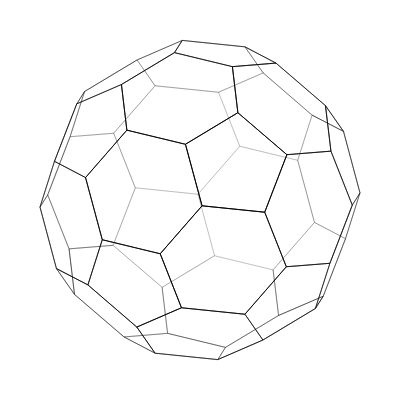
\includegraphics[width=0.2\textwidth]{photos/Buckyball_Carbon.png} 
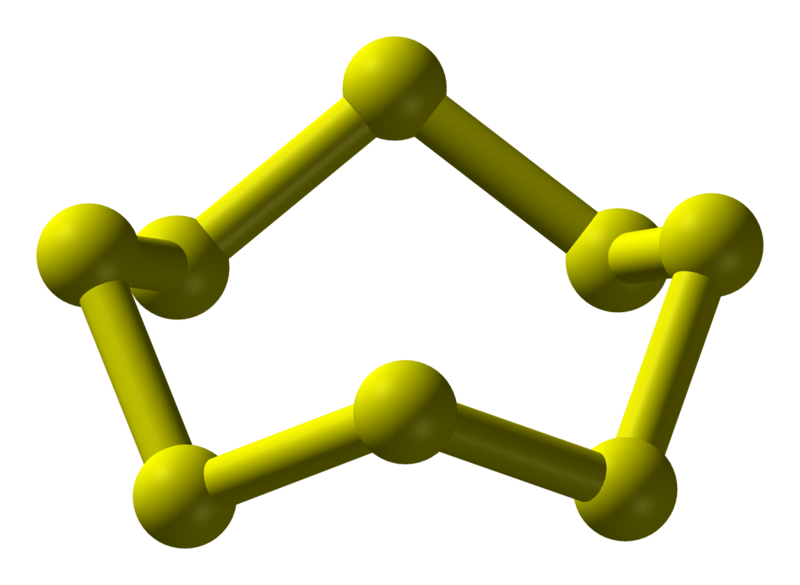
\includegraphics[width=0.2\textwidth]{photos/sulphur_wikipedia.png}
 \end{center}
\caption{Covalent molecular structures}
\end{figure}

\subsection*{Network structures}
Compounds that exist as giant repeating lattice structures ae called network structures. Examples include covalent molecules such as diamond, graphite and silica. Ionic substances are also network structures, for example a sodium chloride crystal is a huge lattice of repeating units made of sodium and chloride ions. All substances formed as a result of ionic bonding are network structures. Metals exist as large continuous lattice structures and are also classified as network structures. For example copper, zinc and iron can be seen as a giant crystals and are therefore considered to be network strucutres.
\begin{figure}[H]
 \begin{center}
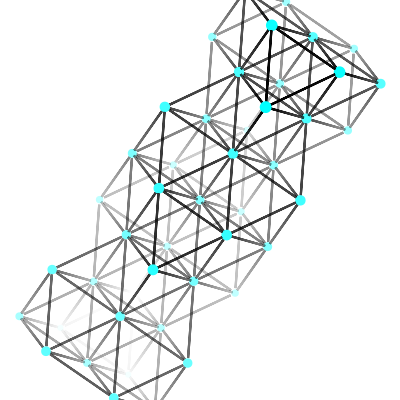
\includegraphics[width=0.2\textwidth]{photos/copper_structure.png} 
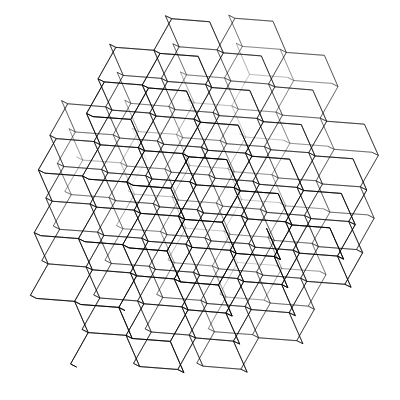
\includegraphics[width=0.2\textwidth]{photos/Diamond_Carbon.png} 
\includegraphics[width=0.2\textwidth]{photos/BaSO4_wikipedia.png} 
 \end{center}
\caption{Network structures. From left to right: metallic, covalent and ionic.}
\end{figure}
            \subsection*{Representing molecules}
            \nopagebreak
        \label{m38120*id307557}The structure of a molecule can be shown in many 
different ways. Sometimes it is easiest to show what a molecule looks like by 
using different types of \textbf{diagrams}, but at 
other times, we may decide to simply represent a molecule using its \textbf{chemical formula} or its written name.\par 
        \label{m38120*id307573}\begin{enumerate}[noitemsep, label=\textbf{\arabic*}. ] 
            \label{m38120*uid2}\item \textbf{Using formulae to show the structure of a 
molecule.}
A \textbf{chemical formula} is an abbreviated 
(shortened) way of describing a molecule, or some other chemical substance. In 
the chapter on classification of matter, we saw how chemical compounds can be 
represented using element symbols from the Periodic Table. A chemical formula 
can also tell us the \textsl{number} of atoms of 
each element that are in a molecule and their \textsl{ratio} in that molecule.
For example, the chemical formula for a molecule of carbon dioxide is
${\mathsf{CO}}_{2}$
The formula above is called the \textbf{molecular 
formula} of that compound. The formula tells us that in one molecule 
of carbon dioxide, there is one atom of carbon and two atoms of oxygen. The 
ratio of carbon atoms to oxygen atoms is 1:2.
\vspace{\rubberspace}\par
        \label{m38120*fhsst!!!underscore!!!id87}
 \Definition{   \label{id2456697}\textbf{ Molecular formula }} { \label{m38120*meaningfhsst!!!underscore!!!id87}
This is a concise way of expressing information about the atoms that make up a 
particular chemical compound. The molecular formula gives the exact number of 
each type of atom in the molecule. 
 } 

A molecule of glucose has the molecular formula:
${\mathsf{C}}_{6}{\mathsf{H}}_{12}{\mathsf{O}}_{6}$.
In each glucose molecule, there are six carbon atoms, twelve hydrogen atoms and 
six oxygen atoms. The ratio of carbon:hydrogen:oxygen is 6:12:6. We can simplify 
this ratio to write 1:2:1 (this means that for every one carbon atom there must be two hydrogen atoms and one oxygen atom), or if we were to use the element symbols, the formula 
would be written as ${\mathsf{CH}}_{2}\mathsf{O}$. This is called the \textbf{empirical formula} of the molecule.
\vspace{\rubberspace}\par
        \label{m38120*fhsst!!!underscore!!!id93}
\Definition{   \label{id2456770}\textbf{ Empirical formula }} { \label{m38120*meaningfhsst!!!underscore!!!id93}
This is a way of expressing the \textsl{relative} 
number of each type of atom in a chemical compound. In most cases, the empirical 
formula does not show the exact number of atoms, but rather the simplest 
\textsl{ratio} of the atoms in the compound. 
 } 

The empirical formula is useful when we want to write the formula for \textsl{network structures}. Since network structures may consist of millions of atoms, it is impossible to say exactly how many atoms are in each unit. It makes sense then to represent these units using their empirical formula. So, in the case of a metal such as copper, we would simply write $\mathsf{Cu}$, or if we were to represent a molecule of sodium chloride, we would simply write $\mathsf{NaCl}$. Chemical formulae therefore tell us something about the \textsl{types} of atoms that are in a compound and the \textsl{ratio} in which these atoms occur in the compound, but they don't give us any idea of what the molecule actually looks like, in other words its \textsl{shape}. To show the shape of compounds we can use diagrams. Another type of formula that can be used to describe a compound is its \textbf{structural formula}. A structural formula uses a graphical representation to show a compound's structure                    
(Figure \ref{fig:representing isobutane}).
    \setcounter{subfigure}{0}
\begin{figure}[h]
\begin{center}
\begin{pspicture}(-5,-1)(5,0.6)
%\psgrid[gridcolor=lightgray]
\rput(-3,0){(a) \textbf{C$_{4}$H$_{10}$}}
\rput(-1,0){(b) \textbf{C$_{2}$H$_{5}$}}
\rput(0.5,0){(c)}
\rput(2,0){\chemfig{CH(-[2]CH_3)(-[7]CH_3)(-[5]CH_3)}}
\end{pspicture}
\caption{Diagram showing (a) the molecular, (b) the empirical and (c) the structural formula of 2-methylpropanone}
\label{fig:representing isobutane}
\end{center}
\end{figure}      
\label{m38120*uid4}\item \textbf{Using diagrams to show the structure of a compound}
Diagrams of compounds are very useful because they help us to picture how the atoms are arranged in the compound and they help us to see the shape of the compound. There are three types of diagrams that are commonly used:
\label{m38120*id307860}\begin{itemize}[noitemsep]
\item \textbf{Wireframe or stick models} \\
In this model, the bonds between atoms are shown as 'sticks'. These 'sticks' are colored to show which atoms are bonding. The common colors that are used are: 
\begin{itemize}[noitemsep]
 \item black or gray for carbon
\item red for oxygen
\item white for hydrogen
\item blue for nitrogen
\item yellow, pink, green for other atoms
\end{itemize}

\label{m38120*uid5}\item \textbf{Ball and stick models} \\
This is a 3-dimensional molecular model that uses 'balls' to represent atoms and 'sticks' to represent the bonds between them. The centres of the atoms (the balls) are connected by straight lines which represent the bonds between them. The balls are colored using the same colors as for the stick or wireframe model.
\item \textbf{Space-filling models} \\
This is also a 3-dimensional molecular model. The atoms are represented by spheres. These spheres are colored as in the stick or wireframe model.
\end{itemize}
Table~\ref{tab:atommodels} shows examples of the different types of models for all the types of compounds.
\begin{table}[H]
 \begin{center}
  \begin{tabular}{|l|l|l|l|l|}  \hline
   & \textbf{Covalent molecular} & \textbf{Covalent network} & \textbf{Ionic network} & \textbf{Metallic network}   \\ \hline
\textbf{Name of compound} & glucose & graphite & silver chloride & zinc \\ \hline
\textbf{Formula} & $\mathsf{C}_{6}\mathsf{H}_{12}\mathsf{O}_6$ or $\mathsf{C}\mathsf{H}_{2}\mathsf{O}$ & $\mathsf{C}$ & $\mathsf{AgCl}$ & $\mathsf{Zn}$  \\ \hline
\textbf{Stick model} & 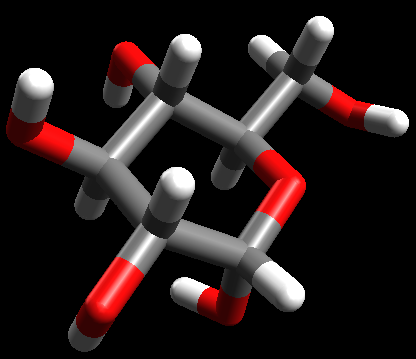
\includegraphics[width=.1\textwidth]{photos/glucose_wire.png} & 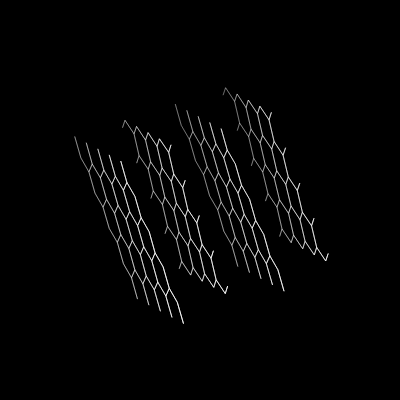
\includegraphics[width=.1\textwidth]{photos/Graphite_Carbon.png} & \scalebox{0.4} % Change this value to rescale the drawing.
{
\begin{pspicture}(0,-1.78)(2.02,1.78)
  \psset{Alpha=75,Beta=20}
  \psset{xMin=-3,xMax=3,yMin=-3,yMax=3,zMin=-3,zMax=3}
%   \pstThreeDCoor
   \pstThreeDLine(-2,-2,-2)(-2,-2,2) \pstThreeDLine(-2,-2,2)(-2,2,2)
   \pstThreeDLine(-2,2,2)(-2,2,-2) \pstThreeDLine(-2,2,-2)(-2,-2,-2)
   \pstThreeDLine(-2,-2,0)(-2,2,0) \pstThreeDLine(-2,0,-2)(-2,0,2)

   \pstThreeDLine(0,-2,-2)(0,-2,2) \pstThreeDLine(0,-2,2)(0,2,2)
   \pstThreeDLine(0,2,2)(0,2,-2) \pstThreeDLine(0,2,-2)(0,-2,-2)
   \pstThreeDLine(0,-2,0)(0,2,0) \pstThreeDLine(0,0,-2)(0,0,2)

  \pstThreeDLine(2,-2,-2)(2,-2,2) \pstThreeDLine(2,-2,2)(2,2,2)
  \pstThreeDLine(2,2,2)(2,2,-2) \pstThreeDLine(2,2,-2)(2,-2,-2)
  \pstThreeDLine(2,-2,0)(2,2,0) \pstThreeDLine(2,0,-2)(2,0,2)

  \pstThreeDLine(-2,2,2)(2,2,2) \pstThreeDLine(-2,0,2)(2,0,2)
  \pstThreeDLine(-2,-2,2)(2,-2,2)
  \pstThreeDLine(-2,2,0)(2,2,0) \pstThreeDLine(-2,0,0)(2,0,0)
  \pstThreeDLine(-2,-2,0)(2,-2,0)
  \pstThreeDLine(-2,2,-2)(2,2,-2) \pstThreeDLine(-2,0,-2)(2,0,-2)
  \pstThreeDLine(-2,-2,-2)(2,-2,-2)
\end{pspicture} 
}  & \includegraphics[width=.1\textwidth]{photos/zinc_sticks.png} \\ \hline
\textbf{Ball-and-stick model} & \includegraphics[width=.1\textwidth]{photos/glucose_balls.png}  & 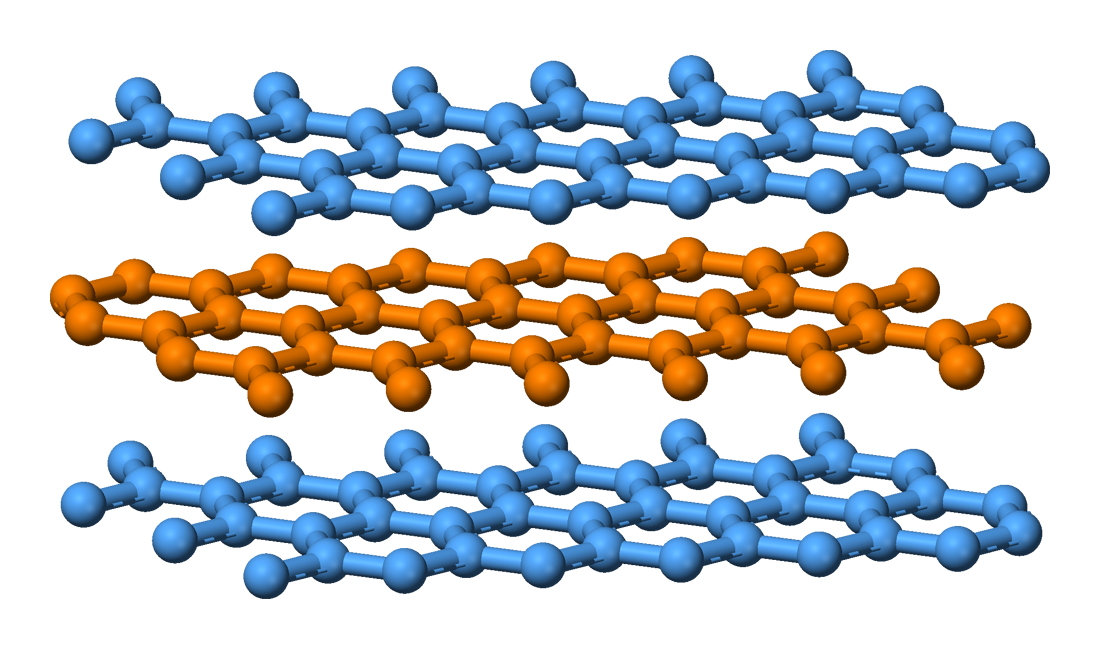
\includegraphics[width=.1\textwidth]{photos/graphite_wikipedia.png} & 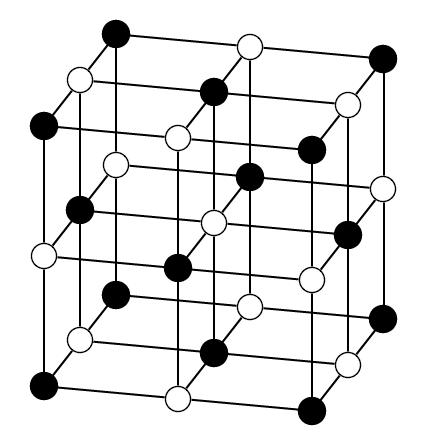
\includegraphics[width=.1\textwidth]{photos/silver_chloride_ballstick.png} & 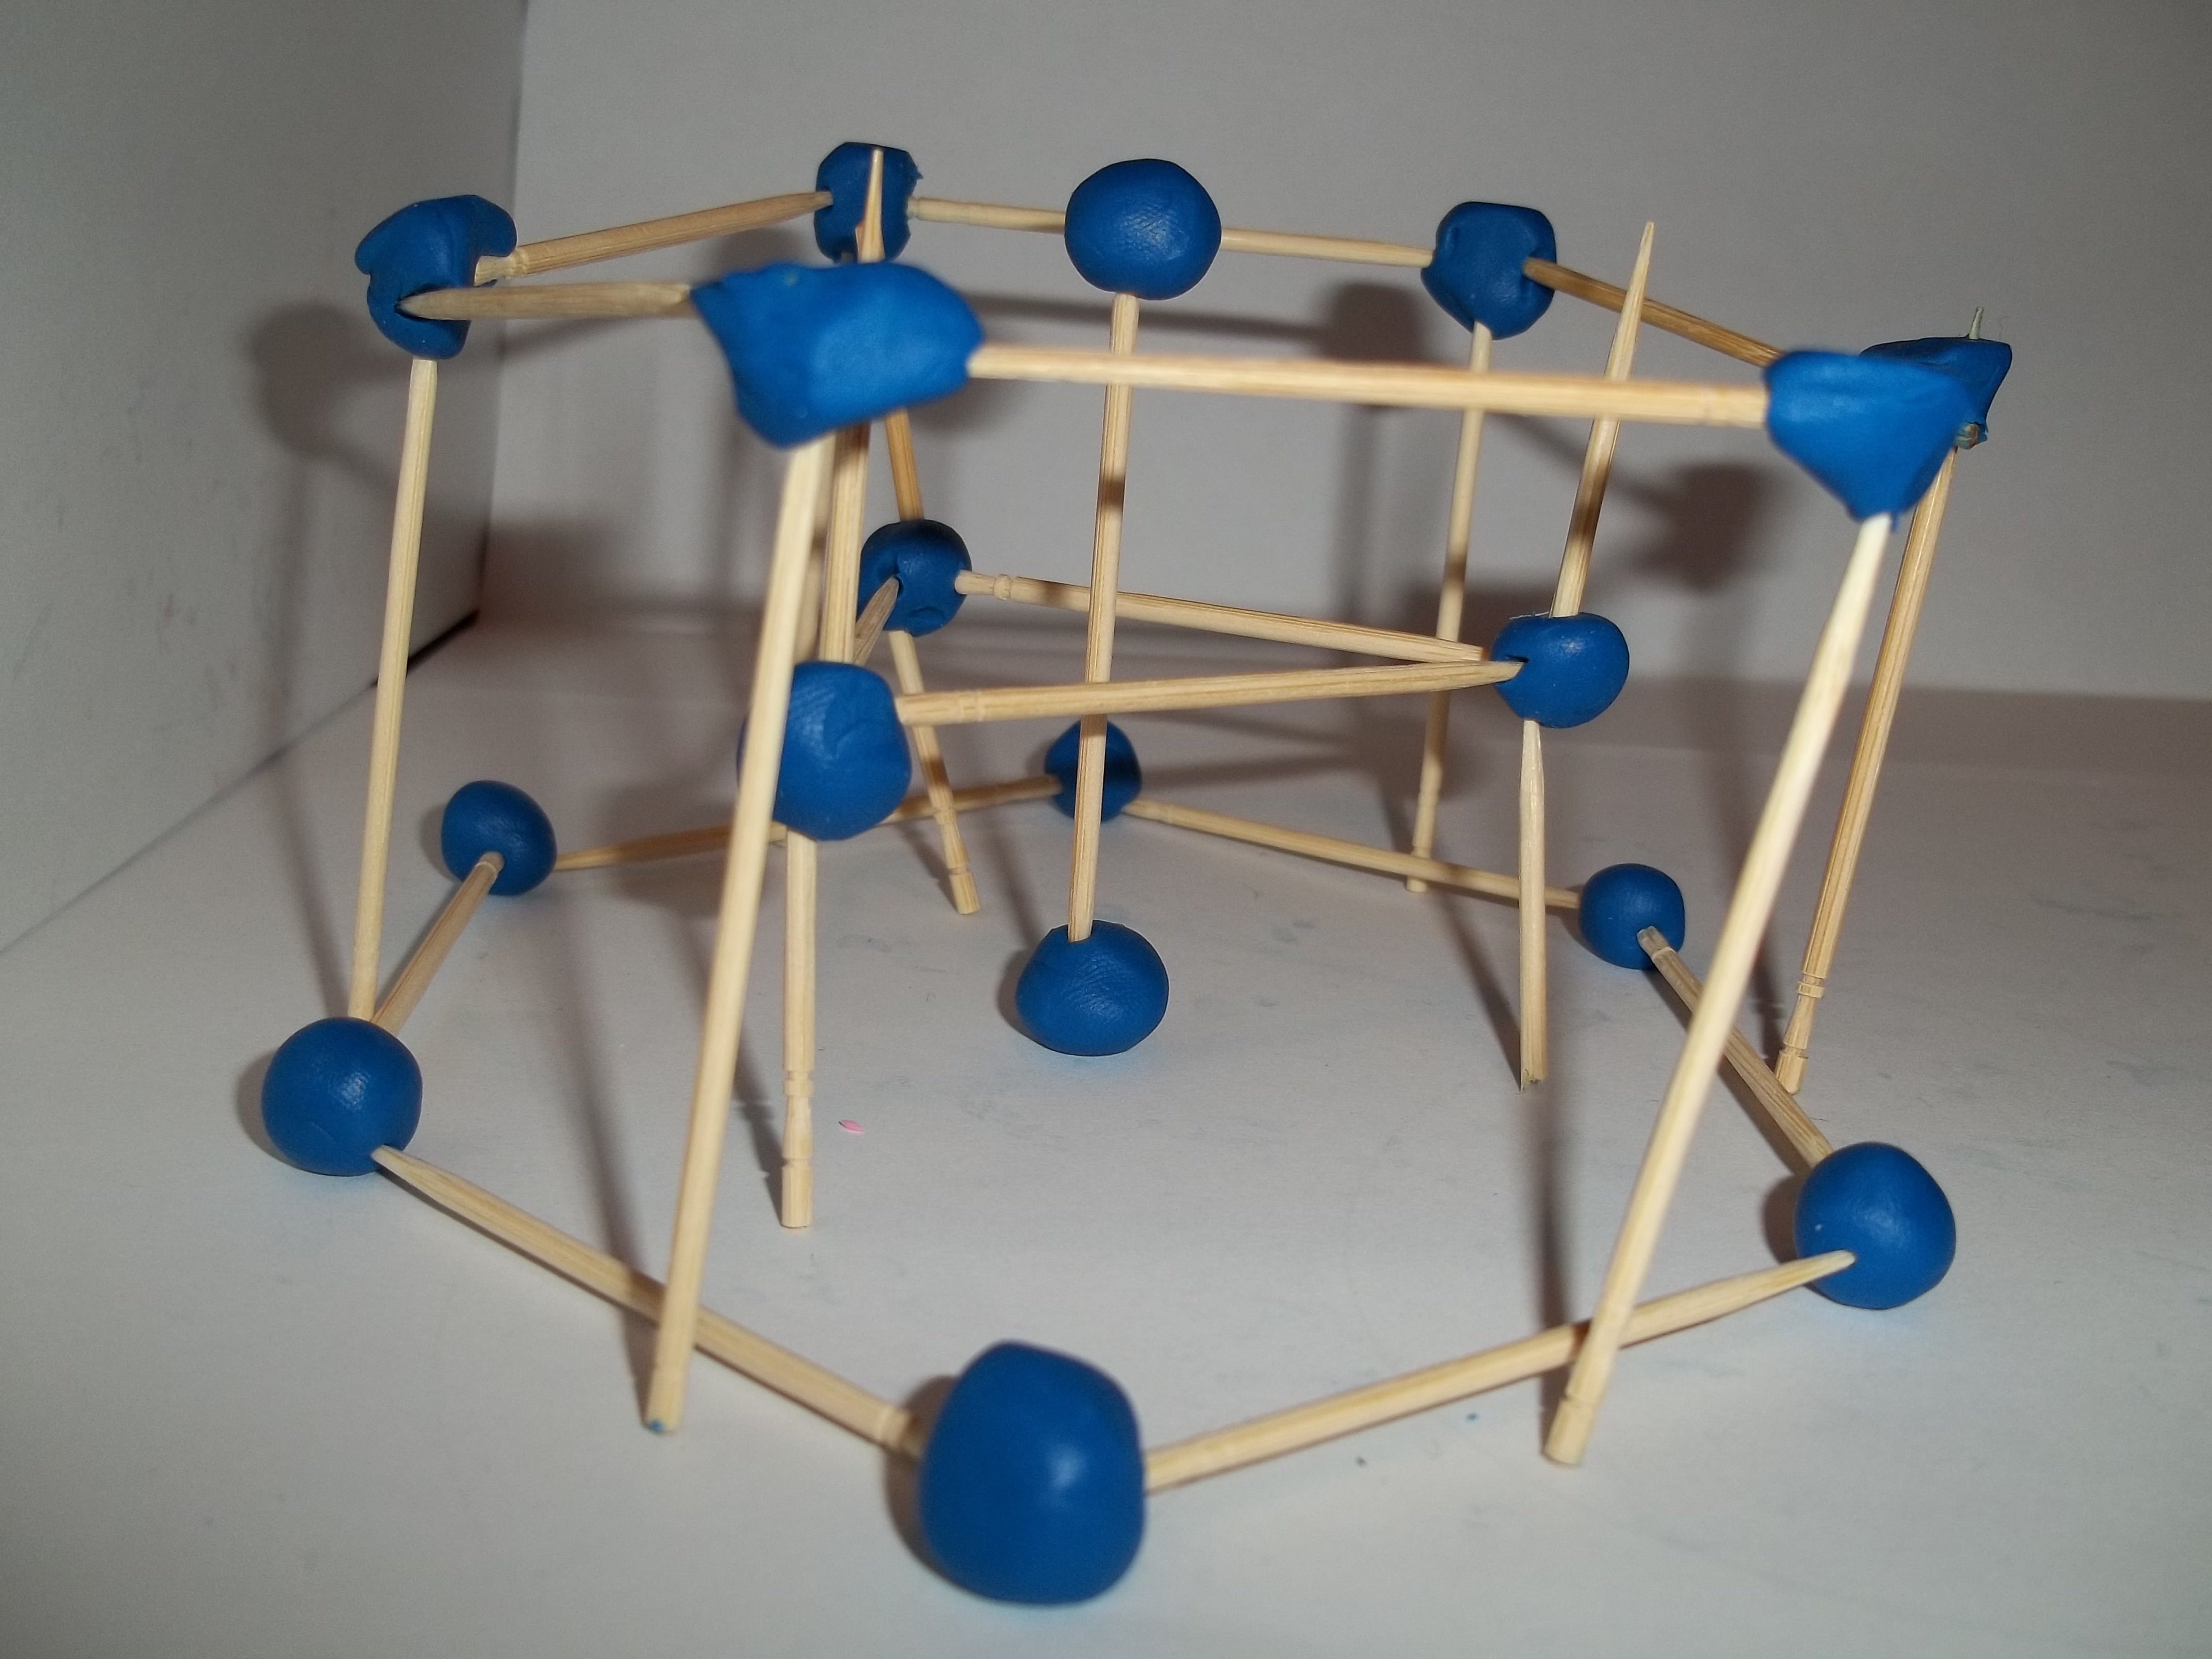
\includegraphics[width=.1\textwidth]{photos/zinc_balls.jpg} \\ \hline
\textbf{Space-filling model} & \includegraphics[width=.1\textwidth]{photos/glucose_spacefill.png}  & 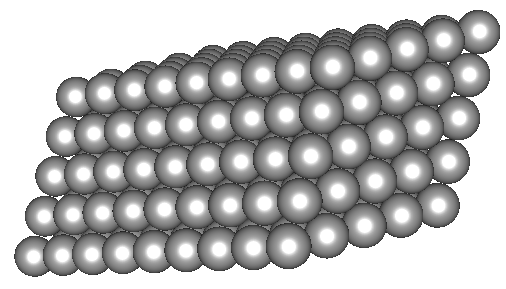
\includegraphics[width=.1\textwidth]{photos/graphite_spacefill.png} & \includegraphics[width=.1\textwidth]{photos/silverchloride_spacefill_wikipedia.png} & 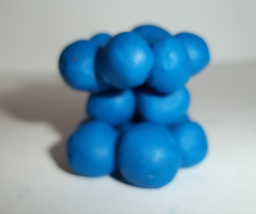
\includegraphics[width=.1\textwidth]{photos/zinc_spacefill.png} \\ \hline
  \end{tabular}
 \end{center}
\caption{Different represetations for compounds}
\label{tab:atommodels}
\end{table}

\begin{Activity}{Representing compounds}
A list of substances is given below. Make use of atomic model kits, play dough and toothpicks, or coloured polystyrene balls and skewer sticks to represent each of the substances in three dimensional structures.\\
\begin{minipage}{.3\textwidth}
\begin{itemize}
 \item glucose ($\mathsf{C}_{6}\mathsf{H}_{12}\mathsf{O}_{6}$)
\item silica ($\mathsf{SiO}_{2}$)
\item sodium chloride ($\mathsf{NaCl}$)
\item sulfur ($\mathsf{S}_{8}$)
\item diamond ($\mathsf{C}$)
\item graphite ($\mathsf{C}$)
\item buckyballs( $\mathsf{C}_{60}$)
\item sucrose ($\mathsf{C}_{12}\mathsf{H}_{22}\mathsf{O}_{11}$)
\item copper ($\mathsf{Cu}$)
\end{itemize}
\end{minipage}
\begin{minipage}{.4\textwidth}
\begin{center}
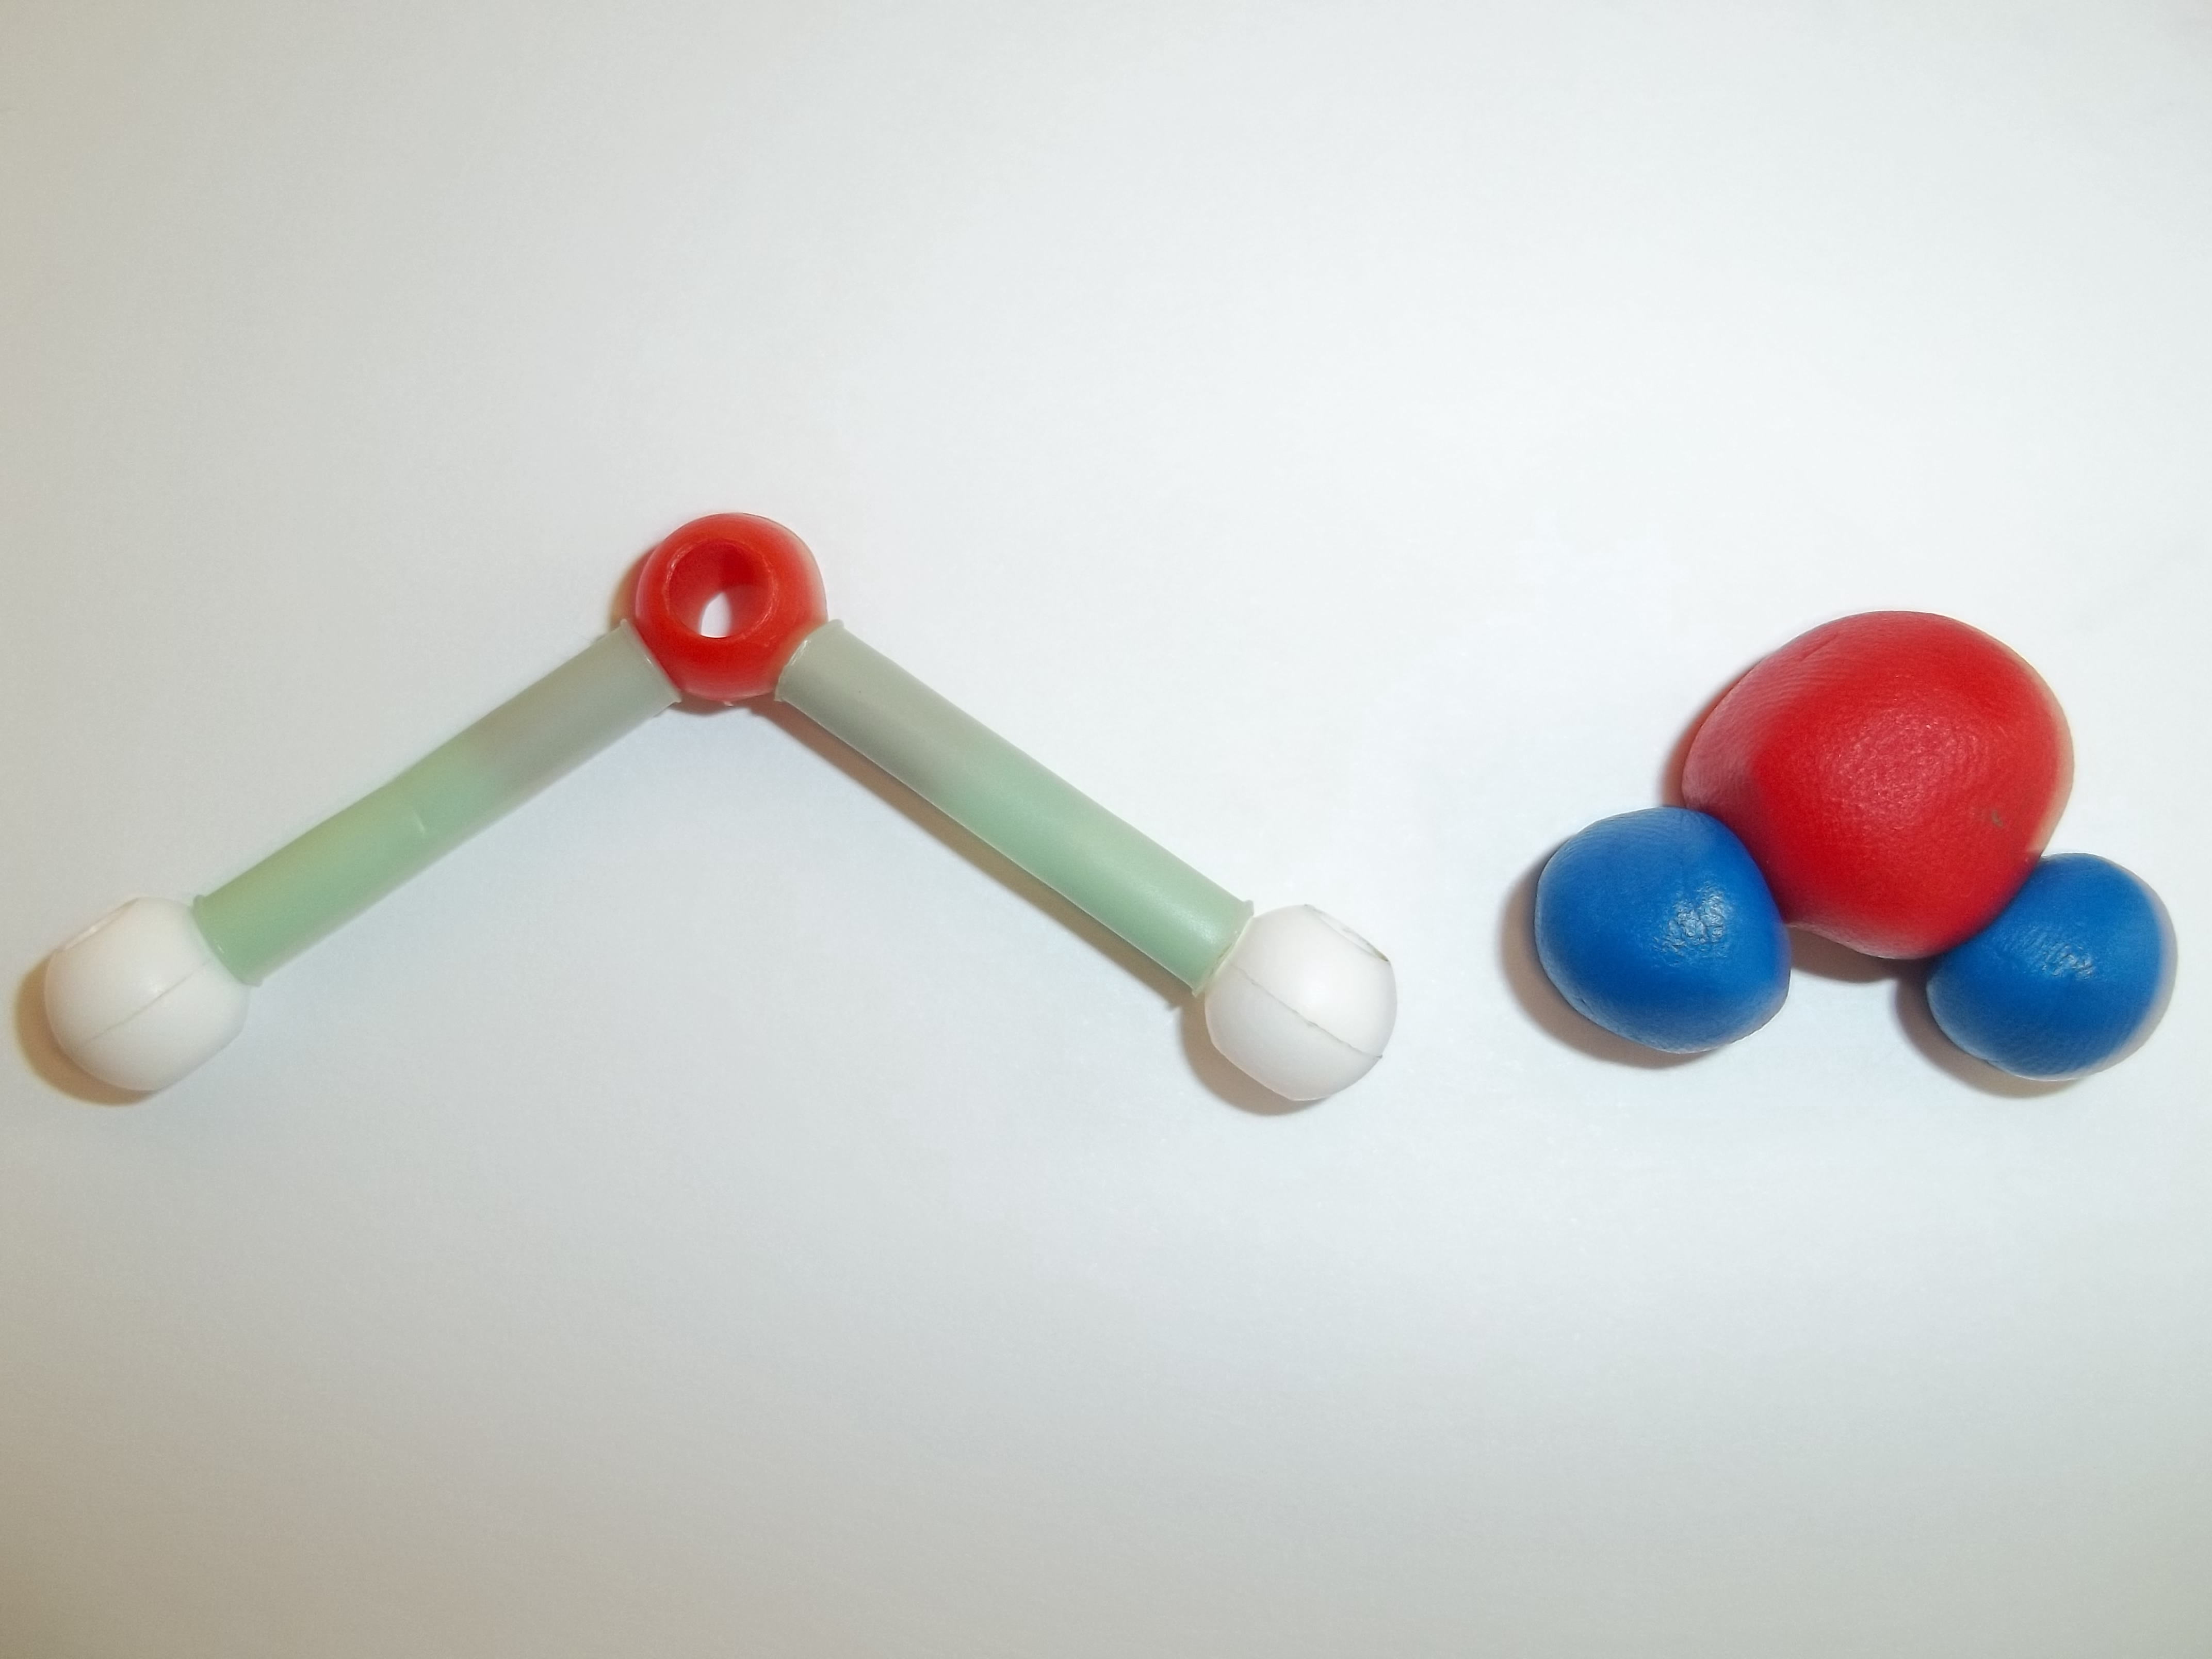
\includegraphics[width=0.6\textwidth]{photos/water.jpg}
\end{center}  
\end{minipage}
\begin{minipage}{.4\textwidth}
\begin{center}
\includegraphics[width=0.6\textwidth]{photos/ammonia.jpg}
\end{center}
\end{minipage}
\end{Activity}
\label{m38120*uid8310432}This website (http://alteredqualia.com/canvasmol/) allows you to view several compounds. You do not need to know these molecules, this is simply to allow you to see one way of representing molecules. 
    \section{ Summary}
            \nopagebreak
            \label{m38120*cid7} $ \hspace{-5pt}\begin{array}{cccccccccccc}   \end{array} $ \hspace{2 pt}\raisebox{-5 pt}{
\includegraphics[width=0.5cm]{col11305.imgs/summary_www.png}} {(section shortcode: P10055 )} \par 
      \label{m38120*id311034}\begin{itemize}[noitemsep]
            \label{m38120*uid67}\item The smallest unit of matter is the \textbf{atom}. Atoms can combine to form \textbf{compounds}.
\label{m38120*uid68}\item A \textbf{compound} is a group of two or more atoms that are attracted to each other by chemical bonds.
\label{m38120*uid69}\item \textbf{Covalent molecular structure} interact and exist as seperate molecules.
\item \textbf{Network structures} exist as giant repeating lattices. Network structures can be covalent, ionic or metallic. 
\label{m38120*uid71}\item The \textbf{chemical formula} of a compound is an abbreviated way of showing a compound, using the symbols for 
the elements in the compound.
\label{m38120*uid72}\item The \textbf{molecular formula} of a molecule gives the exact number of atoms of each element that are in the molecule.
\label{m38120*uid73}\item The \textbf{empirical formula} of a compound gives the relative number of atoms of each element in the compound.
\label{m38120*uid70}\item The structure of a compound can be represented by stick, ball-and-stick or space-filling models.
\item A \textbf{stick} model use colored sticks to represent compounds.
\label{m38120*uid75}\item A \textbf{ball-and-stick} diagram is a 3-dimensional molecular model that uses 'balls' to represent atoms and 'sticks' to represent the bonds between them.
\label{m38120*uid76}\item A \textbf{space-filling model} is also a 3-dimensional molecular model. The atoms are represented by spheres.
\label{m38120*uid77}\item In a molecule, atoms are held together by \textbf{chemical bonds}. Covalent bonds, ionic bonds and metallic bonds are examples of chemical bonds.
\label{m38120*uid78}\item A \textbf{covalent bond} exists between non-metal atoms. An \textbf{ionic bond} exists between non-metal and metal atoms and a \textbf{metallic bond} exists between metal atoms.
\end{itemize}
\label{m38120*secfhsst!!!underscore!!!id497}
            \begin{eocexercises}{Composition of matter}
            \nopagebreak
            \label{m38120*id311490}\begin{enumerate}[noitemsep, label=\textbf{\arabic*}. ] 
            \label{m38120*uid87}\item Give one word or term for each of the following 
descriptions.
\label{m38120*id34411506}\begin{enumerate}[noitemsep, label=\textbf{\alph*}. ] 
            \label{m38120*uid90}\item A composition of two or more atoms that act as a unit.
\label{m38120*uid9221}\item Chemical formula that gives the relative number of atoms 
of each element that are in a molecule.
\end{enumerate}
\label{m38120*uid227}\item Give a definition for each of the following terms: 
\label{m38120*id311506}\begin{enumerate}[noitemsep, label=\textbf{\alph*}. ] 
            \label{m38120*uid930}\item molecule
\label{m38120*uid91}\item ionic compound
\item covalent network structure
\item empirical formula
\item ball-and-stick model\end{enumerate}
\label{m38120*uid92}\item Ammonia, an ingredient in household cleaners, is made up of one part nitrogen ($\mathsf{N}$) and three parts hydrogen ($\mathsf{H}$). Answer the following questions:
\label{m38120*id311590}\begin{enumerate}[noitemsep, label=\textbf{\alph*}. ] 
            \label{m38120*uid94}\item is ammonia a covalent, ionic or metallic substance?
\label{m38120*uid95}\item write down the molecular formula for ammonia
\label{m38120*uid96}\item draw a ball-and-stick diagram
\label{m38120*uid97}\item draw a space-filling diagram
\end{enumerate}
            \label{m38120*uid11}\item In each of the following, say whether the chemical substance is made up of covalent, molecular structures, covalent network structures, ionic network structures or metallic structures:
\label{m38120*id308055}\begin{enumerate}[noitemsep, label=\textbf{\alph*}. ] 
            \label{m38120*uid12}\item ammonia gas (${\mathsf{NH}}_{3}$)
\label{m38120*uid13}\item zinc metal ($\mathsf{Zn}$)
\label{m38120*uid14}\item graphite ($\mathsf{C}$)
\label{m38120*uid15}\item nitric acid (${\mathsf{HNO}}_{3}$)
\label{m38120*uid16}\item potassium bromide ($\mathsf{KBr}$)
\end{enumerate}
\label{m38120*uid17}\item Refer to the diagram below and then answer the 
questions that follow:
    \setcounter{subfigure}{0}
	\begin{figure}[H] % horizontal\label{m38120*id308155}
\begin{center}
\begin{pspicture}(-2.6,-2.4)(6,2)
\SpecialCoor
%\psgrid[gridcolor=lightgray]

\psset{unit=0.75}

\pscircle[fillcolor=red,fillstyle=solid](2,0){1.5}
\pscircle[fillcolor=blue,fillstyle=solid](0,0){2}
\psarc[fillcolor=red,fillstyle=solid](-2,0){1.5}{45}{-45}
\rput(-2,0){\pscurve(1.5;45)(-1.5;180)(1.5;-45)}

\psset{unit=1.5}
\rput(4,0){\pnode(-1,0){RO}\pnode(0,0){C}\pnode(1,0){LO}
\pnode(-1,0.075){ROO}\pnode(0,0.075){CO}\pnode(1,0.075){LOO}
\psline(RO)(C)
\psline(LO)(C)
\psline(ROO)(CO)
\psline(LOO)(CO)
\rput*(C){C}
\rput*(LO){O}
\rput*(RO){O}}
\end{pspicture}
\end{center}
 \end{figure}       \label{m38120*id308161}\begin{enumerate}[noitemsep, label=\textbf{\alph*}. ] 
            \label{m38120*uid18}\item Identify 
the molecule.
\label{m38120*uid19}\item Write the molecular formula for the molecule.
\label{m38120*uid20}\item Is the molecule a covalent, ionic or metallic substance? Explain.
\end{enumerate}
\label{m38120*uid21}\item Represent each of the following molecules using its 
\textsl{chemical formula}, \textsl{structural formula} and the \textsl{ball-and-stick model}.
\label{m38120*id308228}\begin{enumerate}[noitemsep, label=\textbf{\alph*}. ] 
            \label{m38120*uid22}\item hydrogen\label{m38120*uid23}\item ammonia\label{m38120*uid24}\item sulphur dioxide
            \item nitrogen\item carbon dioxide\item methane\item argon\end{enumerate}
\end{enumerate}
  \label{m38120**end}
\par \raisebox{-5 pt}{
\includegraphics[width=0.5cm]{col11305.imgs/summary_www.png}} Find the answers with the shortcodes:
 \par \begin{tabular}[h]{cccccc}
 (1.) l2e  &  (2.) l2M  &  (3.) liV  &  (4.) l2L  &   (1.) li5  &  (2.) liN  &  (3.) liR  \end{tabular}
\end{eocexercises}
